\documentclass[10pt]{article}

\usepackage[margin=0.72in]{geometry}
\usepackage[T1]{fontenc}
\usepackage[utf8]{inputenc}
\usepackage{microtype}
\usepackage{graphicx}
\usepackage{subcaption}
\usepackage{booktabs}
\usepackage{array}
\usepackage{tabularx}
\usepackage[hidelinks]{hyperref}
\usepackage{xcolor}
\usepackage{enumitem}
\usepackage{amsmath}
\usepackage{dblfloatfix}
\usepackage{float}
\usepackage{setspace}

\graphicspath{{../results/arch_compare_20260526/}}

\setlength{\columnsep}{0.22in}
\setlength{\parindent}{0pt}
\setlength{\parskip}{0.45em}
\renewcommand{\arraystretch}{1.12}
\setlist[itemize]{leftmargin=1.2em,itemsep=0.2em,topsep=0.25em}
\makeatletter
\setlength{\@fptop}{0pt}
\setlength{\@fpbot}{0pt plus 1fil}
\setlength{\@fpsep}{8pt}
\makeatother

\definecolor{PaperBlue}{HTML}{203A63}
\definecolor{PaperOrange}{HTML}{F59E0B}
\definecolor{PaperGray}{HTML}{5B6578}
\definecolor{PaperLight}{HTML}{F8FAFC}

\title{\vspace{-1.1em}\bfseries Reference Implementations of 10 Forgetting Attention Mechanisms}
\author{Vuk Rosic\\\small Independent Research Project\\\small Code: \url{https://github.com/vukrosic/forgetting-attention}}
\date{May 26, 2026}

\begin{document}
\maketitle

\begin{abstract}
We describe and implement ten forgetting and memory policies for causal attention and
provide a readable PyTorch reference implementation of each, together with
the training and evaluation infrastructure to scale them to larger models
and longer budgets. As a preliminary check we run the eleven mechanisms
(dense plus ten variants) at three context lengths (2K, 4K, 8K) on an
18M-class LLM transformer for 5 minutes on RTX 3090 each. We also do preliminary experiments. In this small,
unfused setup dense attention leads on loss and throughput; among the
memory variants the simplest ones - block-mean compression, age decay,
hierarchical summaries, surprise retention - cluster at the top. Forgetting mechanism
throughput improves as context length grows: at 2K dense is
roughly twice as fast as the strongest forgetting mechanism, but at 8K
the gap closes to about 15\%, suggesting that further scaling could
flip the ranking in their favor.
\end{abstract}

\begin{figure}[H]
\centering
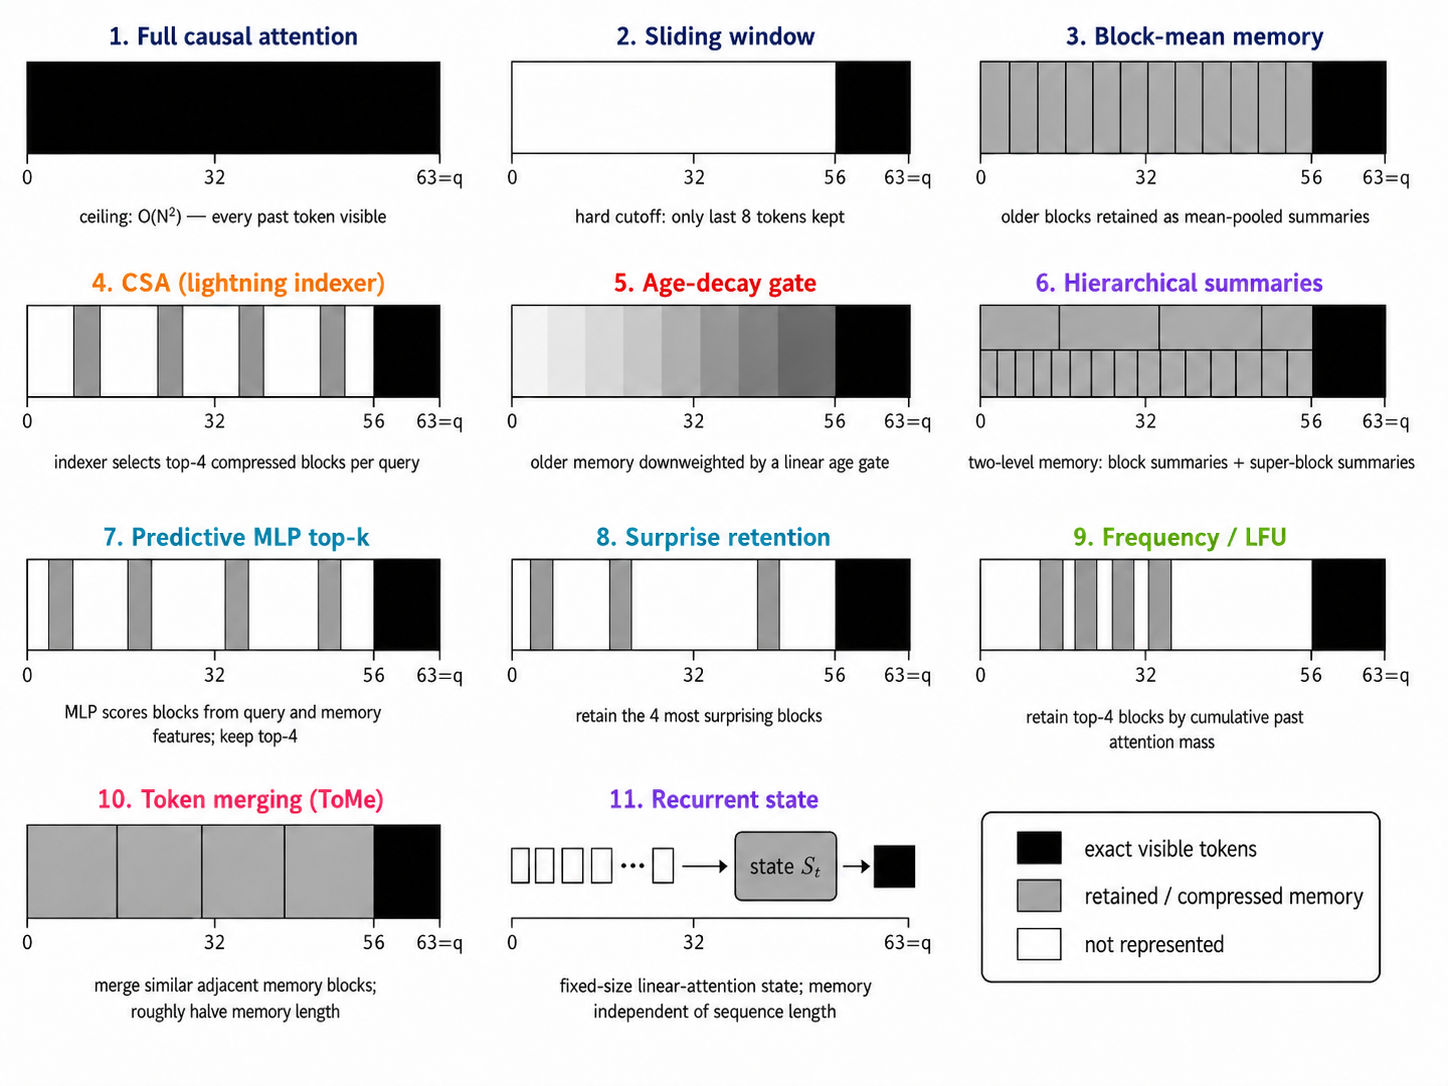
\includegraphics[width=0.82\textwidth]{mechanism_diagrams.png}
\caption{Memory illustration for the mechanisms in this paper. Black
regions are fully visible to the query, gray regions are retained
through memory/gating, and white regions are outside the visible memory.}
\label{fig:diagrams}
\end{figure}

\section{Literature Review}

Long-context transformers usually change one of four things: which
tokens may be attended to, how past state is stored, how old information
is retrieved, or how sequence length is reduced before attention runs.
Local and sparse-attention methods such as Longformer, BigBird,
Reformer, and Routing Transformer reduce the number of keys each query
compares against~\cite{longformer,bigbird,reformer,routing_transformer}.
Memory systems such as Transformer-XL and Compressive Transformer carry
state across segments or compress old states that would otherwise leave
the window~\cite{transformer_xl,compressive_transformer}. Retrieval
methods such as kNN-LM and Memorizing Transformers externalize some of
that memory into a datastore~\cite{knn_lm,memorizing_transformers}.

Modern large models also care about memory compression. DeepSeek-V2 and
DeepSeek-V3 use Multi-head Latent Attention to reduce KV-cache cost at
scale~\cite{deepseek_v2,deepseek_v3}. Our CSA baseline is a small
reference point in that family: old context is still attention material,
but it is represented more cheaply before attention reads it.
Token-merging work such as ToMe motivates a different primitive:
compress redundant content by merging, not only by masking or
dropping~\cite{tome}.

\section{Goal}

\begin{itemize}
\item Provide a reference implementation of ten forgetting-attention policies
ready to scale up by kernel writers and follow-up experiments.
\item Explain each idea clearly with math, code, and a diagram.
\item Provide preliminary analysis and experiment setup.
\end{itemize}

\section{Policies Compared}

Each policy is an alternative per-layer attention module inside the same
transformer block. Figure~\ref{fig:diagrams} shows what each mechanism's
attention pattern looks like at the last query position.

\begin{itemize}
\item \textbf{dense} (classic baseline) --- full causal SDPA with GQA
and RoPE. Every token attends to every earlier token, so cost grows
quadratically with context length.
\item \textbf{local} --- sliding window of $W=64$, no memory. Included as
the isolated baseline so the other policies (which all contain local
attention plus added memory) can be measured against pure local: does
the extra memory machinery add value, or is local doing most of the work?
\item \textbf{compressed\_memory} --- block-mean compression, all blocks
visible, no gate. Distant context is summarized as the mean of each
fixed-size block of keys/values, so each query reads a short summary of
the past plus a fresh local window.
\item \textbf{csa} --- lightning indexer scores compressed blocks; top
$k=4$ kept per query (DeepSeek V4 compressed sparse attention). A small
per-query MLP scores block summaries so that only the highest-ranked
blocks contribute to the output and the rest are masked out.
\item \textbf{age\_forgetting} --- linear age-decay gate: gate $=1-r\cdot
\text{age}$ on compressed blocks. Older summaries lose weight smoothly
until they vanish, giving a soft recency prior without committing to a
hard window cutoff.
\item \textbf{hierarchical} --- two-level: blocks plus
super-blocks-of-blocks, each level gated by $1/(\text{level}+1)$. The
model reads fine local summaries and coarser distant summaries in
parallel, paying less per token the further back the information lies.
\item \textbf{predictive} --- small MLP scores blocks per query from
$(Q, K_b, \text{age})$; top-$k$ kept. Unlike the fixed scoring rules
above, the router learns end-to-end which blocks each query needs.
\item \textbf{surprise\_retention} (new) --- per-block, query-independent
score $s_b = \|V_b - f(K_b)\|^2$ where $f$ is a learned predictor;
top-$k$ most-surprising blocks kept. Blocks whose values are easy to
predict from their own keys are dropped as redundant, so only
information-rich blocks survive.
\item \textbf{frequency\_lfu} (new) --- score is the causal cumulative
sum of past attention mass on each block: blocks the model has actually
used get retained. Retention is self-organizing --- usage during
training determines what stays in memory.
\item \textbf{token\_merge} (new) --- bipartite content-similarity merge
on memory: every other block is paired with its neighbor, top-$r$
most-similar pairs are merged, halving memory length. Adapted from ToMe
in vision: redundancy is compressed by merging similar content, not by
dropping or masking it.
\item \textbf{recurrent\_state} (new) --- linear-attention with positive
feature map $\phi$ and causal cumulative state
$S_t = \sum_{s\leq t} \phi(K_s)\otimes V_s$.
Memory is $O(d_k^2)$ per layer, independent of $T$. Past tokens are
never re-read; they live entirely inside a fixed-size accumulator that
the model rolls forward each step.
\end{itemize}

\section{Correctness Suite}

Each mechanism passes five CUDA tests before entering the sweep:
shape/dtype, causality (future-position perturbations leave earlier
outputs unchanged), mask correctness, gradient flow, and recorded peak
memory. Current status: 55/55 green on one RTX 3090. Run via
\verb|python -m tests.test_forgetting_mechanisms|.

\section{Setup}

\begin{table}[H]
\centering
\small
\caption{Shared experimental setup for the scaling sweep.}
\label{tab:setup}
\begin{tabular}{@{}ll@{}}
\toprule
Item & Value \\
\midrule
Config preset & \texttt{CSAMinimumPaperConfig} \\
Parameters & 18.35M--18.77M \\
Hidden size & 256 \\
Layers / heads & 8 / 8 \\
KV heads (GQA) & 4 \\
Context length sweep & \{2048, 4096, 8192\} \\
Batch size (scaled) & 4 / 2 / 1 (constant tokens/step) \\
Optimizer & Muon (matrix) + AdamW (other) \\
Dataset & \texttt{processed\_data/speedrun\_40M} \\
Hardware & 1$\times$NVIDIA RTX 3090, 24GB \\
Budget per run & 300 active training seconds \\
Eval cadence & every 200 steps \\
Seeds & 1 (this run) \\
\bottomrule
\end{tabular}
\end{table}

\textbf{Fairness rule.} Only the per-layer attention module changes
between rows; model, data, optimizer, seed, and hardware are identical.
Batch size scales with context length so tokens-per-step is constant at
8192, and each run is capped at 300 active training seconds.

\textbf{Metrics.} Each run writes \texttt{metrics.json} with final
validation loss, tokens seen, tok/s, active and wall time, peak
allocated/reserved VRAM, and a per-eval loss history versus tokens and
seconds.

\section{Results}

For our setup (one RTX 3090, 18M-class transformer, 300-second budget,
one seed, unfused PyTorch), the 33-run sweep produces a consistent
pattern across context lengths. Dense leads on both validation loss and
throughput. Local is the strongest cheaper baseline. The
compressed-memory family clusters behind local; CSA and recurrent state
sit further back under this short budget. Among forgetting rules, the
simplest ones do best: age decay and ungated compressed memory at 2K
and 4K, surprise retention at 8K. The learned predictive router and
token-merge variant are weaker here — a signal that extra selection
machinery can lose to simpler memory rules in an unfused, short-budget
setup.

\begin{table}[H]
\centering
\scriptsize
\caption{Completed 33-run sweep. Each row is one 300-second run on the
same RTX 3090. Final loss is not the only fair view because faster
mechanisms process more tokens inside the time cap.}
\label{tab:results}
\resizebox{\textwidth}{!}{\begin{tabular}{@{}llrrrrr@{}}
\toprule
Context & Mechanism & Val loss & Tokens (M) & Tok/s & Time (s) & VRAM GiB \\
\midrule
2048 & \texttt{age\_forgetting} & 4.7595 & 13.9 & 45.7k & 305 & 9.91 \\
2048 & \texttt{compressed\_memory} & 4.7677 & 14.0 & 45.8k & 305 & 9.90 \\
2048 & \texttt{csa} & 5.2627 & 17.7 & 58.3k & 303 & 7.66 \\
2048 & \texttt{dense} & 4.3386 & 37.7 & 124.1k & 304 & 6.94 \\
2048 & \texttt{frequency\_lfu} & 4.7890 & 13.1 & 42.7k & 306 & 9.91 \\
2048 & \texttt{hierarchical} & 4.7589 & 13.9 & 45.4k & 305 & 11.38 \\
2048 & \texttt{local} & 4.5106 & 27.9 & 91.6k & 304 & 7.00 \\
2048 & \texttt{predictive} & 4.8816 & 10.9 & 35.4k & 307 & 12.15 \\
2048 & \texttt{recurrent\_state} & 5.5019 & 18.0 & 59.1k & 305 & 7.00 \\
2048 & \texttt{surprise\_retention} & 4.7906 & 13.4 & 43.7k & 306 & 9.91 \\
2048 & \texttt{token\_merge} & 4.7969 & 12.9 & 42.3k & 306 & 9.89 \\
4096 & \texttt{age\_forgetting} & 4.8268 & 13.1 & 43.1k & 304 & 5.76 \\
4096 & \texttt{compressed\_memory} & 4.8275 & 13.1 & 43.2k & 303 & 5.76 \\
4096 & \texttt{csa} & 5.5567 & 10.3 & 34.1k & 302 & 3.88 \\
4096 & \texttt{dense} & 4.5522 & 26.9 & 89.4k & 301 & 3.51 \\
4096 & \texttt{frequency\_lfu} & 4.8611 & 12.3 & 40.4k & 303 & 5.76 \\
4096 & \texttt{hierarchical} & 4.8367 & 13.1 & 43.2k & 303 & 5.74 \\
4096 & \texttt{local} & 4.6212 & 24.5 & 81.4k & 301 & 3.57 \\
4096 & \texttt{predictive} & 4.9611 & 10.1 & 33.3k & 304 & 6.13 \\
4096 & \texttt{recurrent\_state} & 5.6000 & 15.4 & 50.9k & 303 & 3.54 \\
4096 & \texttt{surprise\_retention} & 4.8577 & 12.7 & 41.9k & 303 & 5.76 \\
4096 & \texttt{token\_merge} & 4.9331 & 10.4 & 34.3k & 303 & 5.75 \\
8192 & \texttt{age\_forgetting} & 5.0689 & 9.8 & 32.5k & 302 & 2.93 \\
8192 & \texttt{compressed\_memory} & 5.0733 & 9.7 & 32.3k & 302 & 2.93 \\
8192 & \texttt{csa} & 5.8409 & 5.0 & 16.7k & 302 & 2.00 \\
8192 & \texttt{dense} & 4.9768 & 13.9 & 46.2k & 301 & 1.80 \\
8192 & \texttt{frequency\_lfu} & 5.1016 & 9.2 & 30.4k & 302 & 2.93 \\
8192 & \texttt{hierarchical} & 5.1066 & 9.0 & 29.9k & 302 & 2.92 \\
8192 & \texttt{local} & 4.9923 & 12.7 & 42.3k & 301 & 1.86 \\
8192 & \texttt{predictive} & 5.1282 & 7.8 & 25.8k & 302 & 3.51 \\
8192 & \texttt{recurrent\_state} & 5.7510 & 11.9 & 39.6k & 302 & 1.82 \\
8192 & \texttt{surprise\_retention} & 5.0660 & 9.2 & 30.6k & 302 & 2.93 \\
8192 & \texttt{token\_merge} & 5.1591 & 7.5 & 24.9k & 302 & 2.92 \\
\bottomrule
\end{tabular}
}
\end{table}

\begin{figure}[H]
\centering
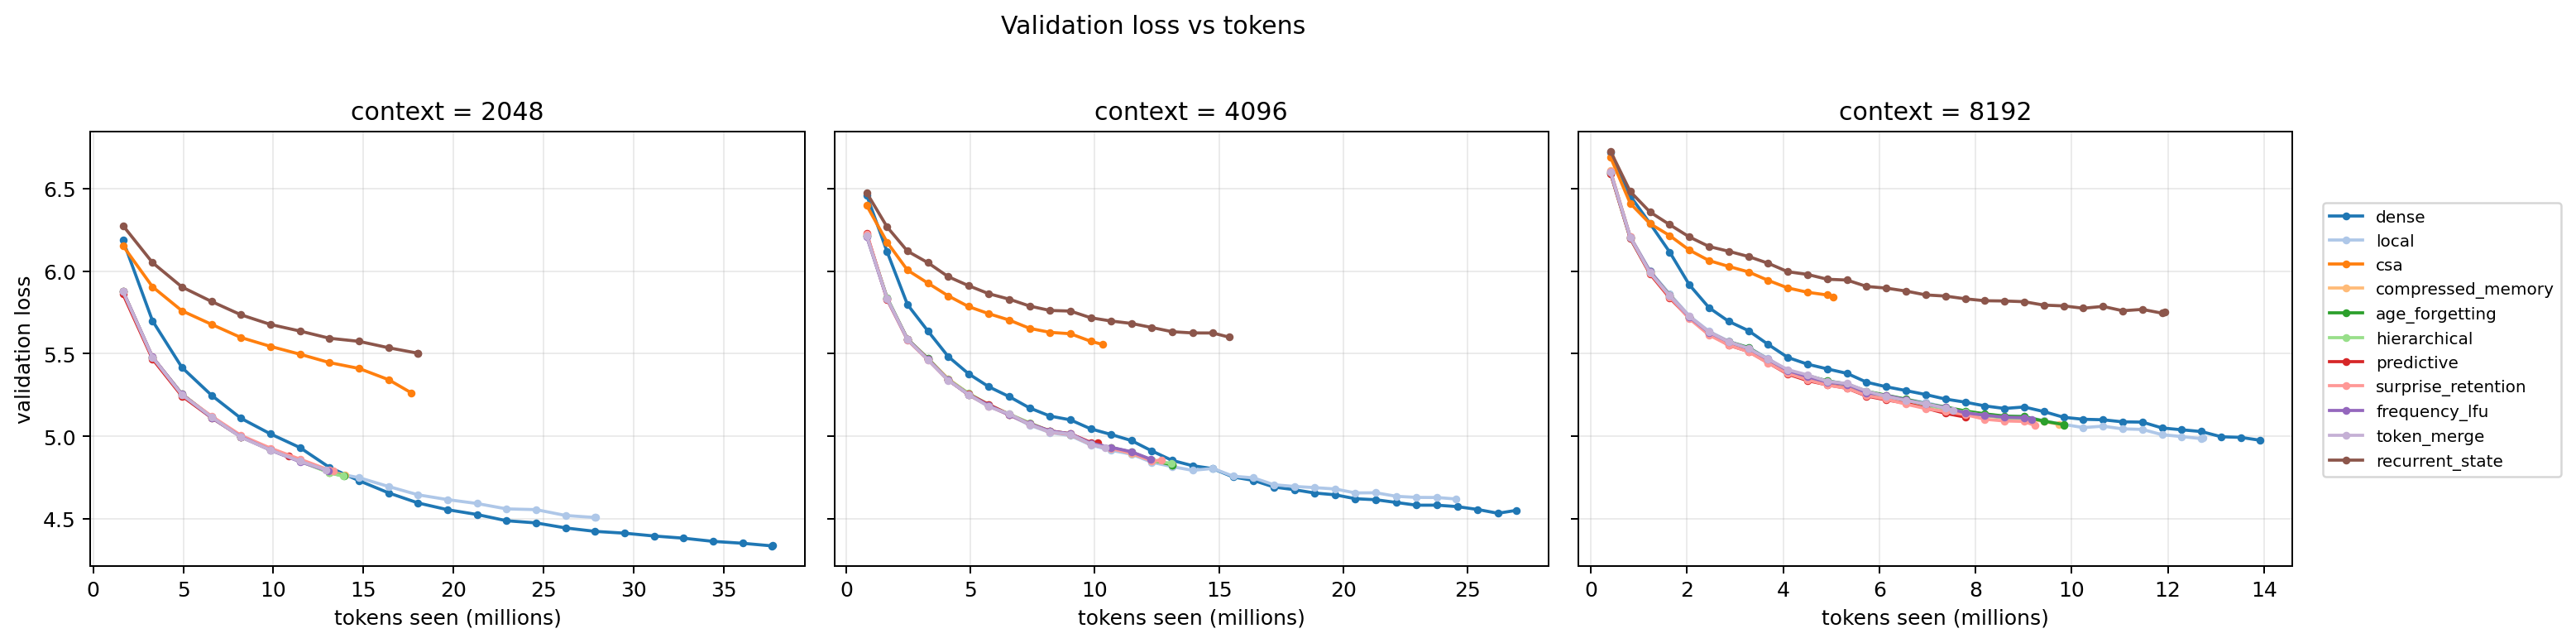
\includegraphics[width=\textwidth]{../results/forgetting_scaling_latest/loss_vs_tokens.png}
\caption{Validation loss vs tokens seen. The fairest curve since the
sweep is time-capped.}
\label{fig:val-loss}
\end{figure}

\begin{figure}[H]
\centering
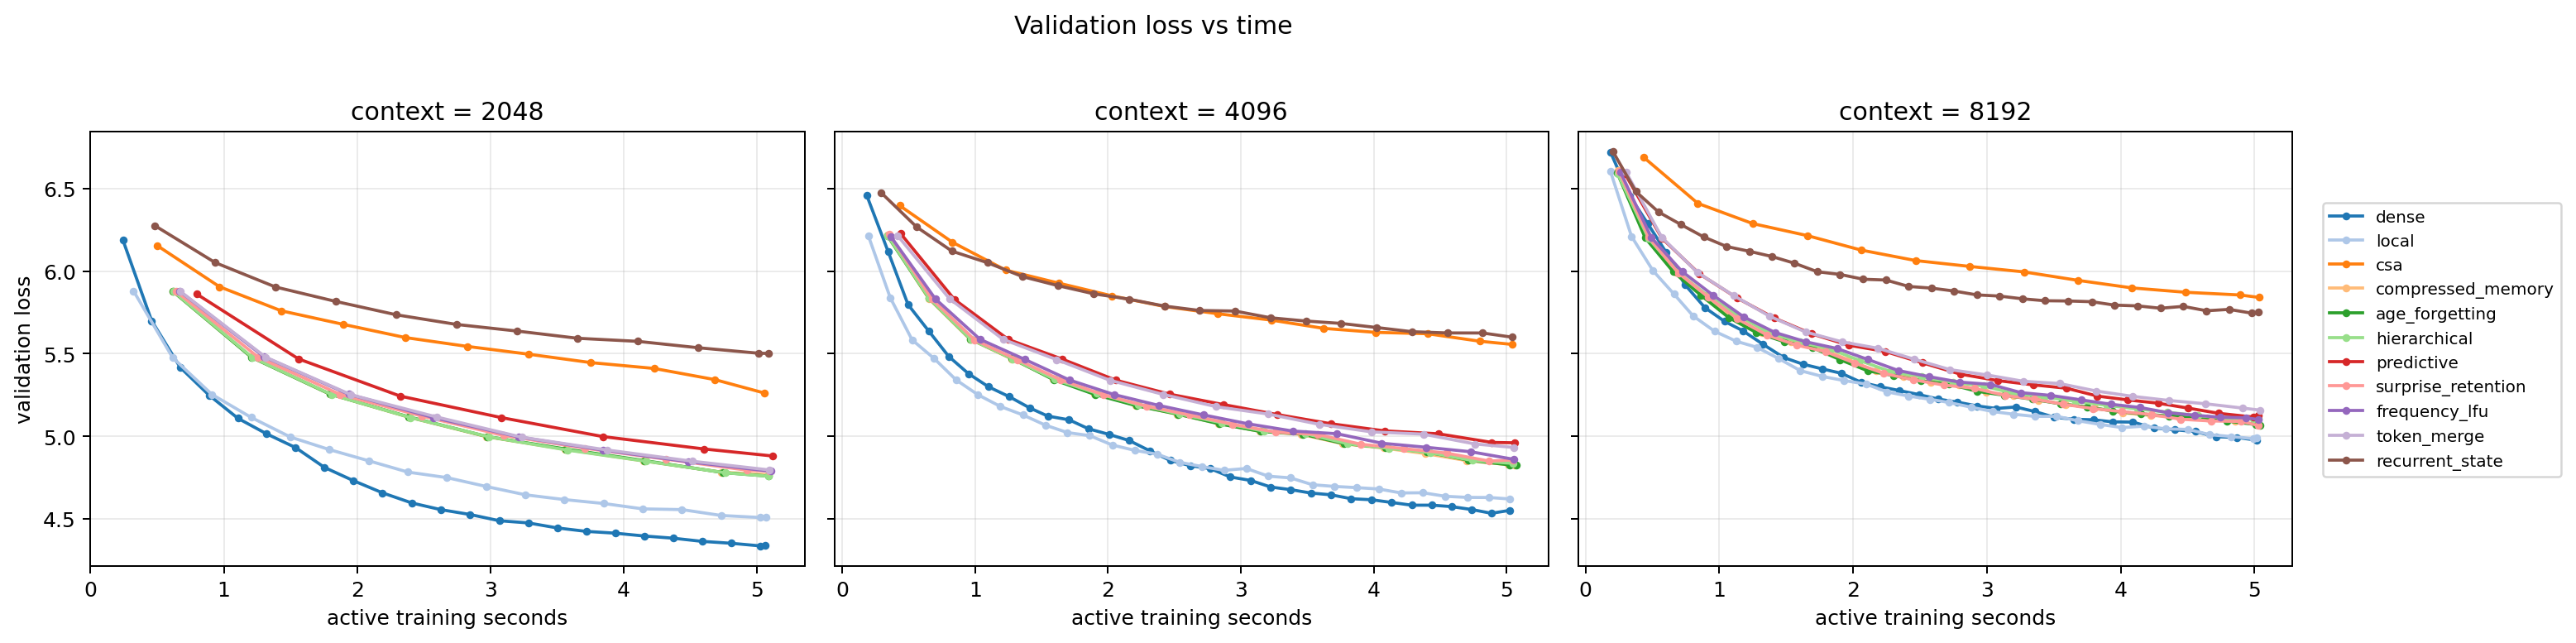
\includegraphics[width=\textwidth]{../results/forgetting_scaling_latest/loss_vs_time.png}
\caption{Validation loss vs active training seconds.}
\label{fig:loss-time}
\end{figure}

\begin{figure}[H]
\centering
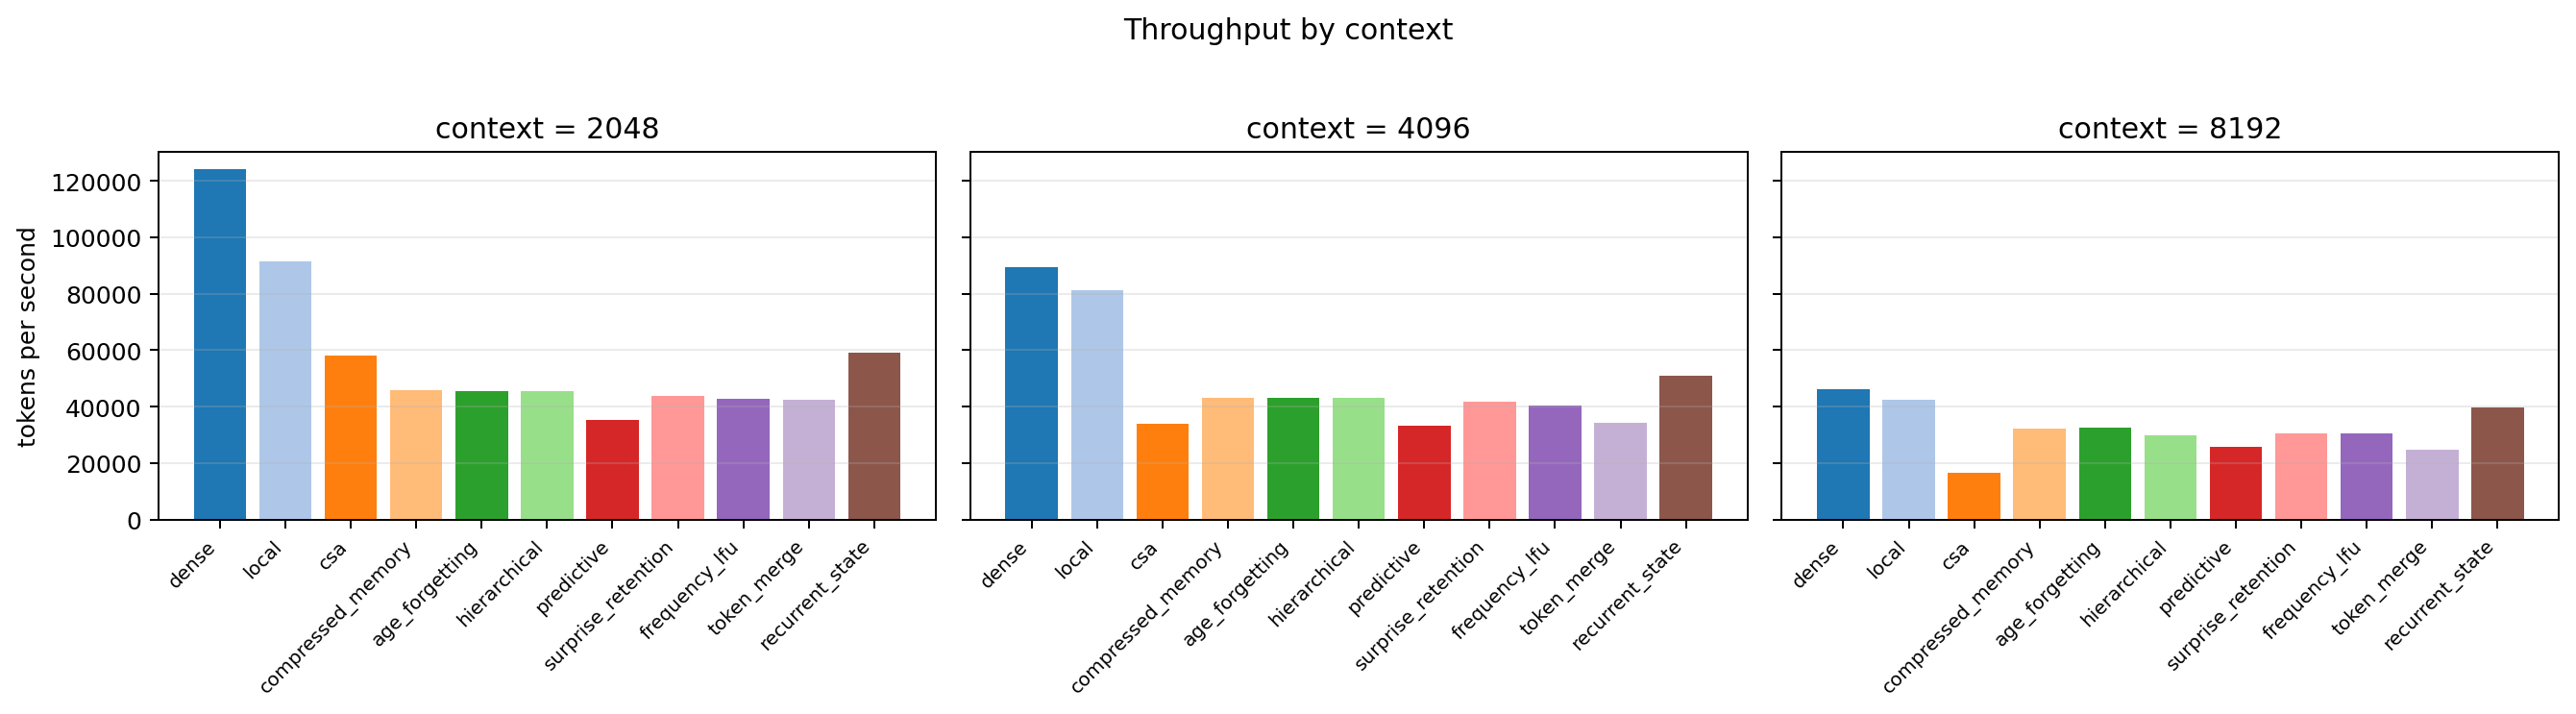
\includegraphics[width=\textwidth]{../results/forgetting_scaling_latest/throughput_by_context.png}
\caption{Throughput (tokens/second) by context length.}
\label{fig:throughput-context}
\end{figure}

\begin{figure}[H]
\centering
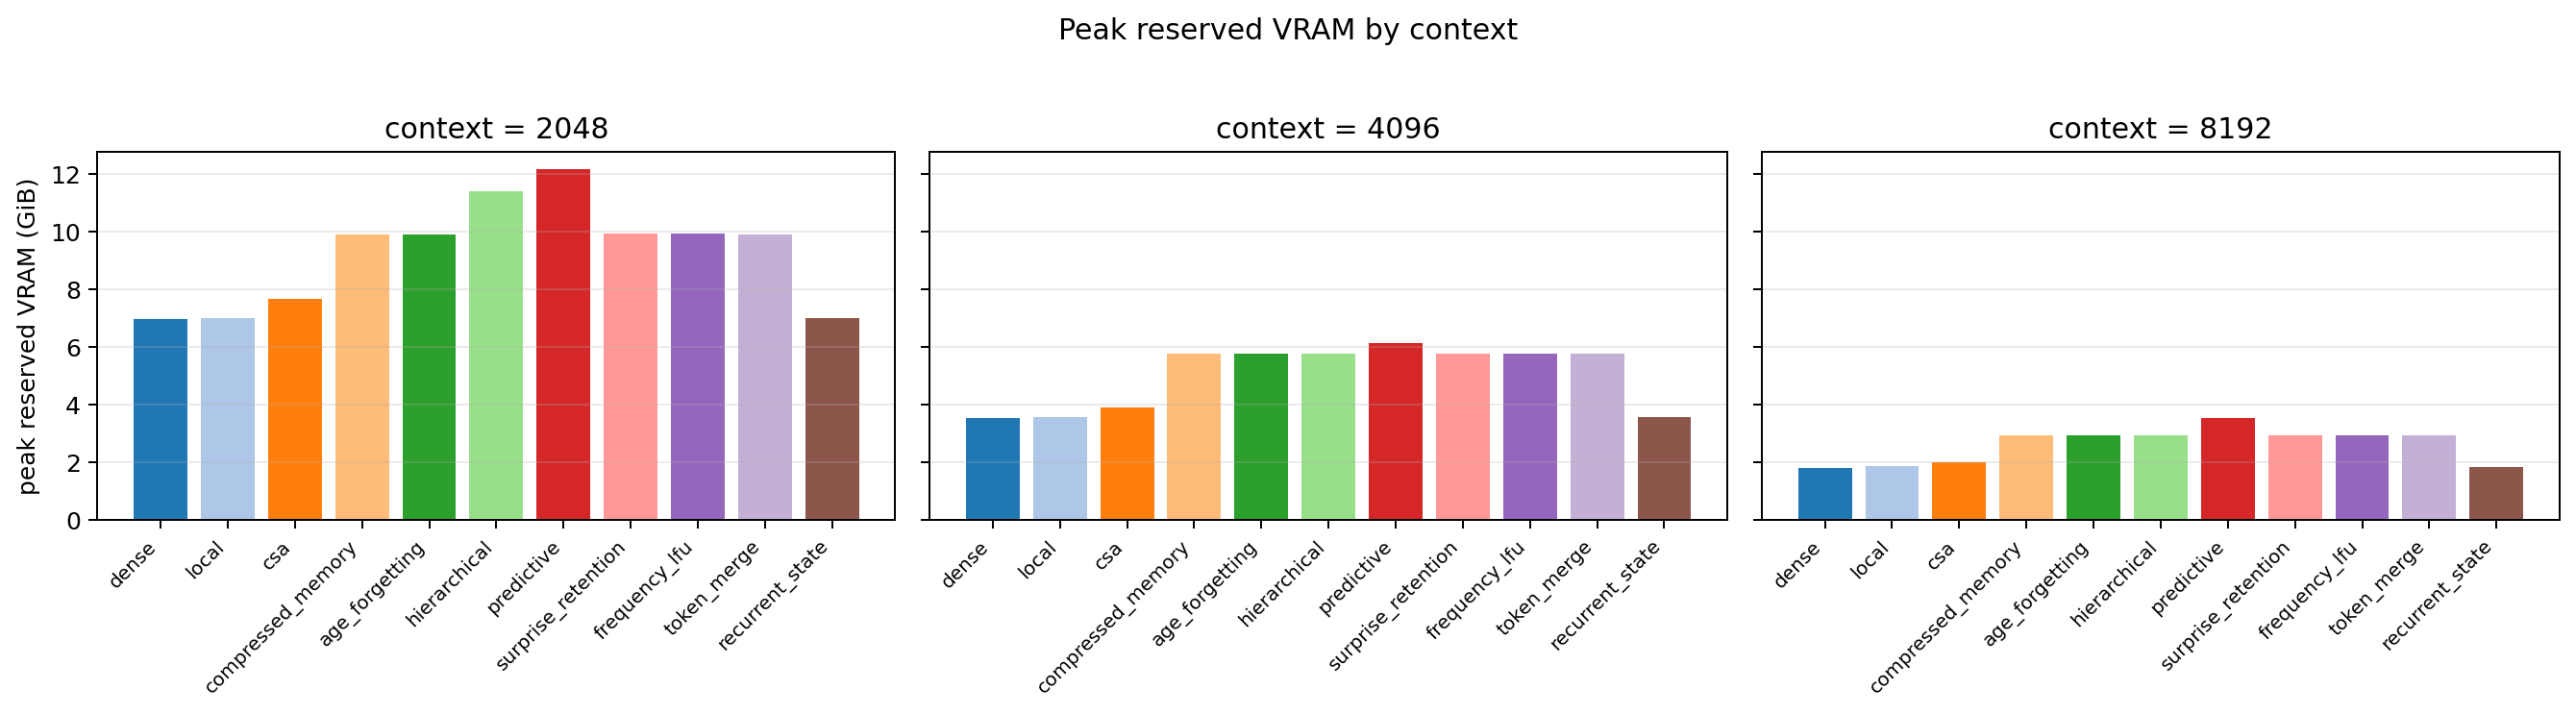
\includegraphics[width=0.85\textwidth]{../results/forgetting_scaling_latest/vram_by_context.png}
\caption{Peak reserved VRAM by context length.}
\label{fig:vram-context}
\end{figure}

\textbf{Takeaway for our setup.} In this reference run the forgetting
policies do not beat dense or local on either metric. But
Figure~\ref{fig:throughput-context} shows the throughput gap closing
fast with context length: at 2K, dense (124K tok/s) is roughly twice as
fast as the strongest forgetting mechanism; at 4K the gap shrinks to
about 1.7$\times$; at 8K, dense (46K tok/s) is only about 15\% ahead of
recurrent state (40K tok/s), and the compressed-memory variants close
in similarly. Dense scales quadratically with sequence length while the
forgetting mechanisms scale closer to linearly, so the natural next
step --- longer contexts or larger models --- is exactly the regime
where these policies are designed to win on throughput, and where the
loss-per-second view (Figure~\ref{fig:loss-time}) should flip in their
favor as a consequence.

\section{Scaling Path}

Each policy is a plain-PyTorch module with math in the docstrings,
paired with a passing causal correctness test, so a kernel writer can
port it to Triton or CUDA, A/B against the reference for exactness, and
rerun the sweep at larger scale. The training script is single-GPU
first but the config, checkpoints, and \texttt{metrics.json} schema
adapt to \texttt{torchrun}, DDP, or an internal harness without code
changes.

\section{Limitations}

One seed, one 3090, one dataset, one parameter scale, unfused kernels.
The numbers describe how each mechanism plateaus on this exact setup.
The task is ordinary next-token prediction, which may not put enough
pressure on the memory system to reveal when old information is useful.
A fused-kernel rerun or a long-memory retrieval task could change the
ranking.

\section{Output Artifacts}

Code: \url{https://github.com/vukrosic/forgetting-attention}. The four
newest mechanisms live in \path{models/new_forgetting.py}, the
correctness suite in \path{tests/test_forgetting_mechanisms.py}, and the
scaling sweep in \path{experiments/forgetting_scaling_sweep.py}.

\section{Conclusion}

The sweep turns ten memory ideas into runnable, causal PyTorch modules
with passing correctness tests and a complete equal-time scaling table.
Dense and local lead on this 18M reference run; among the memory family,
age decay, ungated compressed memory, and surprise retention are the
strongest candidates to fuse and rerun.

\section{Next Steps}

\begin{itemize}
\item Scale compute (larger models, longer budgets, more seeds) and see
which policies remain promising.
\item If any survive scaling, write fused kernels for those paths.
\end{itemize}

\begingroup
\small
\setstretch{0.92}
\setlength{\itemsep}{0pt}
\begin{thebibliography}{13}
\bibitem{deepseek_v2}
DeepSeek-AI.
\newblock {\em DeepSeek-V2: A Strong, Economical, and Efficient Mixture-of-Experts Language Model}.
\newblock 2024.

\bibitem{deepseek_v3}
DeepSeek-AI.
\newblock {\em DeepSeek-V3 Technical Report}.
\newblock 2024.

\bibitem{csaminipaper}
V.~Rosic.
\newblock {\em Can Compressed Sparse Attention Help Under Equal GPU Time?}
\newblock Internal research report, May 24, 2026.

\bibitem{transformer_xl}
Z.~Dai, Z.~Yang, Y.~Yang, J.~Carbonell, Q.~Le, and R.~Salakhutdinov.
\newblock {\em Transformer-XL: Attentive Language Models Beyond a Fixed-Length Context}.
\newblock ACL 2019.

\bibitem{compressive_transformer}
J.~W. Rae, A.~Potapenko, S.~J. Kayumov, and T.~P. Lillicrap.
\newblock {\em Compressive Transformers for Long-Range Sequence Modelling}.
\newblock ICLR 2020.

\bibitem{longformer}
I.~Beltagy, M.~E. Peters, and A.~Cohan.
\newblock {\em Longformer: The Long-Document Transformer}.
\newblock arXiv:2004.05150, 2020.

\bibitem{bigbird}
M.~Zaheer et al.
\newblock {\em Big Bird: Transformers for Longer Sequences}.
\newblock NeurIPS 2020.

\bibitem{reformer}
N.~Kitaev, L.~Kaiser, and A.~Levskaya.
\newblock {\em Reformer: The Efficient Transformer}.
\newblock ICLR 2020.

\bibitem{routing_transformer}
A.~Roy, M.~Saffar, A.~Vaswani, and D.~Grangier.
\newblock {\em Efficient Content-Based Sparse Attention with Routing Transformers}.
\newblock TACL 2021.

\bibitem{memorizing_transformers}
Y.~Wu, M.~N. Rabe, D.~Hutchins, and C.~Szegedy.
\newblock {\em Memorizing Transformers}.
\newblock ICLR 2022.

\bibitem{knn_lm}
U.~Khandelwal, O.~Levy, D.~Jurafsky, L.~Zettlemoyer, and M.~Lewis.
\newblock {\em Generalization through Memorization: Nearest Neighbor Language Models}.
\newblock ICLR 2020.

\bibitem{tome}
D.~Bolya, C.-Y.~Fu, X.~Dai, P.~Zhang, C.~Feichtenhofer, J.~Hoffman.
\newblock {\em Token Merging: Your ViT But Faster}.
\newblock ICLR 2023.

\bibitem{linear_attn}
A.~Katharopoulos, A.~Vyas, N.~Pappas, F.~Fleuret.
\newblock {\em Transformers are RNNs: Fast Autoregressive Transformers with Linear Attention}.
\newblock ICML 2020.
\end{thebibliography}
\endgroup

\end{document}
